\subsection[Mainflux]{Mainflux}
Mainflux jak większość platform IoT umożliwia połączenie urządzeń do aplikacji oraz jednocześnie zapewni bezpieczeństwo na wysokim poziomie. Tak jak było przedstwione w  tabeli powyżej mainflux oferuje wieloprotokołowy przekaźnik komunikatów, pozwala to na wybranie odpowiedniego protokołu do zapewnienia niezbędnych wymagań.
Mainflux jest używany jako oprogramowanie pośrednie onznacza to, że wykorzystuje serwer (SW) który udostępnia funkcje oraz usługi które są potrzebne przy przy tworzeniu aplikacji IoT. podstawowymi usługami są: 

\begin{itemize}
    \item Messaging bridge (HTTP Sender, MQTT and WS, CoAP) – pośredniczy w wysyłaniu wiadomości pomiędzy urządzeniem a aplikacją. 
    \item User manager (Mainflux UI, Mainflux CLI) – umożliwia użytkownikowi zarządzanie zasobami. Pierwszy sposób to zarządzanie przez stronę internetową (Mainflux UI). Aby użytkownik mógł zarządzać zasobami musi się zalogować na stronie, po czym ma możliwość dodawania, usuwania, educji rzeczy oraz łączenia kanałów z rzeczami. Drugim sposobem jest bootstraping (Mainflux UI) czyli zautomatyzowany ….
    \item Normalizer -
    \item NATS – otrzymuje wiadomości od rzeczy i może automatycznie reagować na przesłane dane, w oparci o konfigurowalny zestaw reguł.
\end{itemize}

poniższy schemat pokazuje zależności między tymi usługami 

\begin{figure}[H]
    \centering
    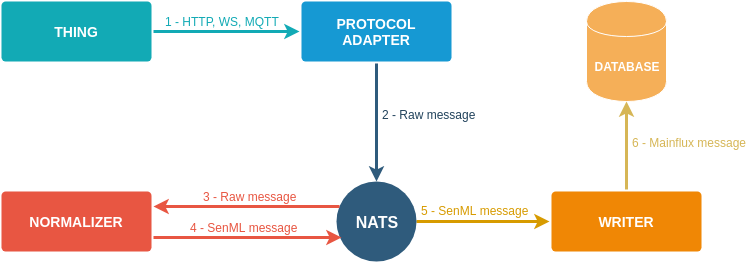
\includegraphics[width=\textwidth]{kp03}
    \caption{Placeholder}
    \label{fig:iotarch}
\end{figure}
//https://medium.com/mainflux-iot-platform/mainflux-open-source-iot-platform-set-up-and-usage-70bed698791a 

Aby zrozumieć jak działa przesyłanie wiadomości za pośrednictwem platformy mainflux trzeba poznać trzy podstawowe koncepty jakie zostały wprowadzone.
\begin{itemize}
    \item Urzytkownik (eng. user)- reprezentuje człowieka w systemie, który jest identyfikowany za pomocą danych do logowania jest on używany do zarządzania innymi zasobami. Zarządzanie obejmuje tworzenie, edytowanie oraz usuwanie rzeczy  i kanałów, a także do łączenia rzeczy z kanałami. 
    \item Rzecz (eng. Thing) - reprezentuje urządzenie lub aplikację każda rzecz posiada identyfikator oraz klucz dodatkowo, może mieć przypisany typ (aplikacja, urządzenie). 
    \item Kanał (eng. Channel)- pozwala na połączenia rzeczy między sobą. Każdy kanał ma swoje id, do kanału może być podłączonych więcej niż 2 rzeczy, każdy kto nasłuchuje na danym kanale otrzymuje tą wiadomość.
\end{itemize}

